\documentclass[11pt]{article}
\usepackage[margin=0.8in]{geometry}
\usepackage{bm}
\usepackage{amsfonts}
\usepackage{amsthm}
\usepackage{amssymb}
\usepackage{amsmath}
\usepackage{xcolor}
\usepackage{tikz}
\usepackage[colorlinks = true]{hyperref}

\usepackage{fancyhdr}
\pagestyle{fancy}
\fancyhf{}
\lhead{UNSW Business School}
\rhead{ACTL3182 Cheatsheet}
\cfoot{Page \thepage}  %PERHAPS Add UNSW COPYRIGHT FOOTER
\setlength{\headheight}{17pt} 

\title{\textbf{ACTL3182 Cheatsheet}}
\author{Andrew Wu}
\date{September 2021}

\usepackage{titlesec}
\titleformat{\section}{\Large\sffamily\bfseries\color{red}}{\thesection}{0.5em}{}[]
\titleformat{\subsection}{\color{red!75}\large\sffamily\bfseries}{\thesubsection}{0.5em}{}
\titleformat{\subsubsection}{\color{red!50}\normalsize\sffamily\bfseries}{\thesubsubsection}{0.5em}{}

\newcommand{\E}{\mathbb{E}}
\newcommand{\F}{\mathcal{F}}
\newcommand{\PR}{\mathbb{P}}
\renewcommand{\Pr}{\mathbb{P}}
\newcommand{\R}{\mathbb{R}}
\newcommand{\Cov}{\operatorname{Cov}}
\newcommand{\Q}{\mathcal{Q}}

\begin{document}
	\maketitle
	\textbf{NOTE:} Theory sections are written to simplify the text for easy revision. Yours answers to exam questions may need to be more detailed than what is written here. This cheatsheet may be revised throughout the term, please check \url{https://github.com/BrownianNotion/ACTL3182_21T3.git} for the latest version.
	\section{Modern Portfolio Theory}
	\subsection{Utility Theory}
	\subsubsection{Utility Axioms}
	The expected utility theorem is a consequence of the following axioms:
	\begin{enumerate}
		\item \textbf{Completeness (Comparability):} For all decisions \( A,B \), either \( A \prec B \), \( A\succ B \) or \( A\sim B \)
		\item \textbf{Transitivity:} If \( A\succ B \) and \( B\succ C \), then \( A\succ C \)
		\item \textbf{Independence:} If \( A\sim B \) then for any \( C \), 
		\[	G(A,C;\alpha) \sim G(B, C; \alpha)\]
		\item \textbf{Measurability:} If \( A\succ B\succ C \), there exists a unique \( \alpha \) such that
		\[ B\sim G(A, C;\alpha)	\]
		\item \textbf{Ranking:} Suppose \( A\succ B\succ D \), \( A\succ C\succ D \), \( B\sim G(A, D;\alpha_1) \) and \( C\sim G(A, D; \alpha_2) \). Then, if \( \alpha_1\geq\alpha_2 \), then \( B\succ C \).
		\item \textbf{Certainty Equivalent:} All gambles have a price.
	\end{enumerate}

	\subsubsection{Expected Utility Theorem}
	Assuming the utility axioms, \( W_1 \) is preferred over \( W_2 \) iff \( \E[U(W_1)] \geq \E[U(W_2)] \)
	
	\subsubsection{Non-Satiation}
	Individuals always prefer more wealth to less: \( U'(w) > 0 \).
	\subsubsection{Investor types}
	\begin{center}
		\def\arraystretch{1.25}
	\begin{tabular}{lcccc}
		\hline
		\hline
		\textbf{Type} & \textbf{Wealth Preference} & \textbf{Utility Preference} & $\bm{U''}$ & \textbf{Concavity}\\
		\hline
		Risk-Averse & \( \E[W] \succ W \) & \( U(\E[W]) > \E[U(W)] \) & \( U'' < 0 \) & concave\\
		\hline
		Risk-Neutral & \( \E[W] \sim W \) & \( U(\E[W]) = \E[U(W)] \) & \( U'' = 0 \) & linear\\
		\hline
		Risk-Lover &\( \E[W] \prec W \) & \( U(\E[W]) < \E[U(W)] \) & \( U'' > 0 \) & convex\\
		\hline
		\end{tabular}
	\end{center}
	\subsubsection{Risk Premium}
	The amount \( \pi(W) \) that an individual will pay to give up risk:
		\[	\pi(W) = \E[W] - c(W)\]
	where \( c(W) := U^{-1}(\E[U(W)]) \) is the \textbf{certainty wealth equivalent}.
	\subsubsection{Risk Aversion}
	Absolute risk aversion \( A(w) \) and relative risk aversion \( R(w) \)
	\[	A(w) = -\frac{U''(w)}{U'(w)},\quad R(w) = -w\frac{U''(w)}{U'(w)}.\] 
	If \( A(w) \) is decreasing, then an investor invests more \( \$ \) in risky assets as wealth increases.\\If \( R(w) \) is decreasing, an investor invests a higher proportion of wealth in risky assets as wealth increases.
	\subsection{Investment Risk Measures}
	\subsubsection{Definition}
	A function \( \mathcal{\theta}: X\to\R\) that summarises an investment's risk with a single number.
	\subsubsection{Common Examples}
	\begin{enumerate}
		\item Variance: \( \int_{-\infty}^{\infty} (x - \mu)^2 f_{X}(x)dx \)
		\item Downside-Variance: \( \int_{-\infty}^{\mu} (x - \mu)^2 f_{X}(x)dx \)
		\item Shortfall Probability: \( \PR(X \leq L ) \)
		\item Expected Shortfall: \( \int_{-\infty}^{L}(L-x)f_{X}(x)dx \)
		\item Shortfall Variance: \( \int_{-\infty}^{L}(L-x)^2  f_{X}(x)dx \)
	\end{enumerate}
	\subsubsection{Value-at-Risk:}
	The Value-at-risk \textbf{at level }\( \bm{\alpha} \) is the maximum possible loss from holding a portfolio over a \textbf{given time period} so that the \textbf{probability of a larger loss is} \(\bm{1 - \alpha}  \).\\
	In general, 
	\[	\text{VaR}(\alpha) = \mu - X_{1 - \alpha},
		\]
	where \( X_{1-\alpha} \) is the \( (1 - \alpha) \)-quantile of X.
	If \( X\sim\mathcal{N}(\mu, \sigma^2) \), then 
	\(	\text{VaR}(\alpha) = \sigma Z_{\alpha}
		\).
	\subsection{Portfolio Optimisation}
	\subsubsection{Two assets}
	Global Minimum Variance Portfolio: \[	w_A = \frac{\sigma^2_B - \sigma_{AB}}{\sigma^2_A + \sigma^2_B - 2\sigma_{AB}},\quad w_B = 1 - w_A\]
	Portfolio Variance:
	\[	\sigma_P^2 = w_A^2 \sigma_A^2 + w_B^2 \sigma_B^2 + 2w_A w_B\sigma_{AB}\]
	
	\subsubsection{N-risky assets}
	Minimise \( \displaystyle\sigma_P^2 = \bm{w}^{\top} \Sigma \bm{w} \), \( \quad \)subject to \( \bm{1}^{\top}\bm{w}= 1 \) and \( \bm{z}^{\top}\bm{w}=\mu \).\\[5pt]
	Lagrangian: \( \mathcal{L}(\bm{w}, \lambda, \gamma)  = \frac{1}{2} \bm{w}^{\top} \Sigma \bm{w} + \lambda (1 - \bm{1}^{\top}\bm{w}) + \gamma (\mu - \bm{z}^{\top}\bm{w})\)\\\\
	Constants: \begin{align*}
				&	A = \bm{1}^{\top}\Sigma^{-1}\bm{1},\quad B =  \bm{1}^{\top}\Sigma^{-1}\bm{z} = \bm{z}^{\top}\Sigma^{-1}\bm{1}\\[2pt]
				&	C = \bm{z}^{\top}\Sigma^{-1}\bm{z}, \quad\Delta = AC - B^2\\
				\end{align*} 
	%\\[5pt]
	Minimum Variance Portfolio: 
	\[ \displaystyle\bm{w} = \lambda \Sigma^{-1} \bm{1} + \gamma \Sigma^{-1}\bm{z}  \]where \[ \lambda = \frac{C - B\mu}{\Delta}, \quad\gamma = \frac{A \mu- B}{\Delta} \]\\\\
	%\\[5pt]
	Portfolio Variance: \[ \sigma_P^2 = \frac{A\mu^2 -2B\mu + C}{\Delta} \]\\
	Global Minimum Variance Portfolio: \[ \bm{w}_g = \frac{1}{A}\Sigma^{-1}\bm{1} \]
	
	\subsubsection{N-risky assets + risk-free}
	Minimise \( \sigma_P^2 = \bm{w}^{\top} \Sigma \bm{w} \), \( \quad \)subject to \( (\bm{z} - r_{f}\bm{1})^{\top}\bm{w} = u - r_f \).\\[5pt]
	Lagrangian: \( \mathcal{L}(\bm{w}, \lambda, \gamma)  = \frac{1}{2}\bm{w}^{\top}\Sigma\bm{w} + \gamma(\mu - r_f - (\bm{z} - r_f \bm{1})^{\top}\bm{w}) \)\\\\
	Minimum Variance Portfolio: \[ \bm{w} = \gamma\Sigma^{-1}(\bm{z} - r_f \bm{1}) \] where \[ \gamma = \frac{\mu - r_f}{A r_f^2 -2B r_f + C} \]\\\\
	Portfolio Variance: \[ \sigma_P^2 = \frac{(\mu - r_f)^2}{A r_f^2 -2B r_f + C} \]\\\\
	Tangency Portfolio: \[ \bm{w}_t = \gamma_t \Sigma^{-1}(\bm{z} - r_f \bm{1}) \] where \[ \gamma_t = \frac{1}{B - Ar_f} \]
	\newpage
	\subsubsection{Two Fund Theorem (N-risky assets)}
	All efficient portfolios are a linear combination of any two efficient portfolios. 
	\subsubsection{One Fund Theorem (N-risky + risk-free)}
	All efficient portfolios are a linear combination of the tangent portfolio and the risk-free asset.
	
	\newpage
	%%%%%%%%%%%%%%%%%%%%%%%%%%%%%%%%%%%%%%%%%%%%%%%%%%%%%%%%%%%%%%%%%%%%%%%%%%%%%%%%%%%%%%%%%%
	\section{Asset Pricing Models}
	For all parts in section 2, \( i \) takes values \( 1,2,... N \) and indexes the assets in the market.
	\subsection{CAPM}
	\subsection{CAPM Assumptions}
	\begin{enumerate}
		\item Investors choose optimal portfolios based only on the mean and variance of returns. Justified if returns are normally distributed returns or utility functions are quadratic.
		\item Homogeneity: Investors agree on the distribution of returns and plan over a single common period.
		\item No Market Frictions (eg. taxes, short-selling restrictions, restricted information)
		\item Investors can borrow or lend without limit at the risk-free rate.
		\item Market Portfolio consists of all publicly traded assets.
	\end{enumerate}
	\subsubsection{Capital Market Line}
	%The line representing all efficient portfolios when there are \( N \)-risky assets and a risk-free asset.
	\[	\mu_{e} = r_{f} + \frac{\sigma_{e}}{\sigma_{M}}(\mu_{M} - r_{f})\]
	%where \( {}_{e}, {}_{M} \) denote the efficient and Market Portfolios respectively.
	\subsubsection{Security Market Line}
	
	\begin{align*}
	&\mu_i = r_f + \beta_i (\mu_M - r_f), \quad\text{where} \\[4pt]
	&\beta_i = \frac{\sigma_{i, M}}{\sigma_{M}^2}
	\end{align*}	
	\subsubsection{Risk Decomposition}
	\begin{align*}
		\sigma_i^2 & = \beta_i^2 \sigma_M^2 + \sigma_{\xi_{i}}^2 \\
		& = \text{Systematic Risk} + \text{Non-systematic Risk}
	\end{align*}	
	\subsection{Factor Models}
	\subsubsection{Single Factor Model (SFM)}
	\[	r_i = \alpha_i + \beta_i f + \epsilon_i, \]
	where \( \alpha_i, \beta_i \) are stock-specific constants, \( f \) is the factor capturing market-wide price movement and \( \epsilon_i \) is a noise term reflecting firm-specific risk.
	\subsubsection{SFM Assumptions}
	\begin{enumerate}
		\item \( (r_i, f) \) are jointly normal
		\item \( \epsilon_i\sim\mathcal{N}(0, \sigma_{\epsilon_i}^2) \)
		\item \( \Cov(\epsilon_i, f) = 0 \)
		\item \( \Cov(\epsilon_i, \epsilon_j) = 0 \) for \( i\neq j \)
	\end{enumerate}
	\subsubsection{Risk Decomposition and Covariance}
	\begin{align*}
	& \sigma_i^2 = \beta_i^2 \sigma_f^2 + \sigma_{\epsilon_{i}}^2 = \text{Systematic Risk} + \text{Non-systematic Risk}\\
	& \sigma_{i, j} = \beta_i \beta_j \sigma_f^2
	\end{align*}
	\subsubsection{Diversification}	
	\[	R_P^2 = \frac{\beta_P^2 \sigma_f^2}{\sigma_P^2} = \frac{\text{Systematic Risk}}{\text{Total Risk}}\]
	Full diversification when \( R_P^2 = 1 \).
	\subsubsection{Multi-Factor Models}
	\[	r_i = \alpha_i + \beta_{i, 1}f_1 + \beta_{i, 2}f_2 + ... + \beta_{i, K} f_K + \epsilon_i \]
	Factors \( f_i \) may include inflation, economic growth, interest rates etc.
	\subsection{APT}
	\subsubsection{Assumptions}
	Replace rigid CAPM assumptions with more relaxed assumptions:
	\begin{enumerate}
		\item No arbitrage in the market
		\item Large universe of securities
		\item Returns follow a factor model
	\end{enumerate}
	\subsubsection{Single-Factor APT Assumptions}
	Assume returns follow the following factor model:
		\[	r_i = \alpha_i + \beta_{i}I+\epsilon_{i}\]
	Define the standardised factor \( f:=(I - \mu_{I})/\sigma_{I} \) (\( \sim\mathcal{N}(0,1) \)) and assume:
	\begin{enumerate}
		\item \( \E[\epsilon_i] = 0 \)
		\item \( \Cov(\epsilon_i, \epsilon_j) = 0\) if \( i\neq j \)
		\item \( \Cov(\epsilon_i, I) = 0\)
		\item Unlimited short-selling
	\end{enumerate}
	\subsubsection{Single-Factor APT Returns}
	\begin{align*}
		& r_i = a_i + b_i f + \epsilon_i\\[5pt]
		& \E[r_i] = a_i,\quad \sigma_i^2 = b_i^2 + \sigma_{\epsilon_i}^2,\quad\sigma_{i, j} = b_{i}b_{j}
	\end{align*}
	Under no-arbitrage, 
	\[	a_i = \lambda_0 + \lambda_1 b_i,\]
	where \( \lambda_0 = r_f \) if there is a risk-free asset. The \( \lambda_i \)'s are called factor prices.
	\subsubsection{Multi-Factor APT Returns}
	\[	r_i = a_i + b_{i,1 }f_1 + b_{i,2} f_2 + ... + b_{i, K}f_K + \epsilon_i\]
	where
	\[	\E[r_i] = a_i = \lambda_0 + \lambda_1 b_{i,1} + \lambda_2 b_{i, 2} + ... + \lambda_K b_{i, K}\]
	and \( \lambda_0 = r_f \) if there is a risk-free asset. 
	\subsection{Market Efficiency}
	%\subsubsection{Estimating returns}
	%Using historical data to estimate mean return is not feasible: over 100 years of data would be needed to get a reliable estimate.
	\subsubsection{Investment approaches}
	\begin{enumerate}
		\item Technical analysis: Analyse historical data (price and volume).
		\item Fundamental analysis: Measure intrinsic value of stocks and compare with market price.
		\item Efficient market selection: Define acceptable risk level and form broad portfolio.
	\end{enumerate}
	\subsubsection{Types of market efficiency}
	\begin{enumerate}
		\item Strong form: Market prices reflect all information including insider information.
		\item Semi-strong form: Market prices reflect all publicly available information %(fundamental and technical analysis are useless).
		\item Weak form: Market prices reflect all historical data 
		%(technical analysis is useless).
	\end{enumerate}
	\newpage
	%%%%%%%%%%%%%%%%%%%%%%%%%%%%%%%%%%%%%%%%%%%%%%%%%%%%%%%%%%%%%%%%%%%%%%%%%%%%%%%%%%%%%%%%%
	\section{Discrete Time Derivative Pricing}
	\subsection{Options}
	Let: \( S_t \) denote the time \( t \) stock price, \( c_t, p_t \) denote the time \( t \) European call/put prices, \( T \) denote the option's maturity, \( K \) denote its strike price and \( r \) denote the risk-free rate.
	\subsubsection{Vanilla Options}
	A vanilla European call/put gives the holder the right \textbf{but not obligation} to buy/sell the asset at maturity \( T \) for strike price \( K \). American options are defined the same way except they can be exercised at \textbf{any time up to maturity}.
	\begin{center}
		\begin{tabular}{ccc}
			\hline
			\hline
			\textbf{Moneyness} & \textbf{European Call} & \textbf{European Put} \\
			\hline
			In the money & \( S_T > K \) & \( S_T < K \)\\
			\hline
			At the money & \( S_T = K \) & \( S_T = K \)\\
			\hline
			Out of the money &  \( S_T < K \)& \( S_T > K \)\\
			\hline
			\end{tabular}
		\end{center}
	\subsubsection{Payoff Functions and Price Bounds}
	Define \( 0\leq U\leq T \) as the exercise time for an American option. \( U:=\infty \) if option not exercised. \\Note: \( (X)_{+} := \max\{0, X\} \). Option bounds are for option prices at \textbf{time} \( \bm{t} \).
	\begin{center}
		\def\arraystretch{1.25}
		\begin{tabular}{lccc}
			\hline
			\hline
			\textbf{Option} & \textbf{Payoff} & \textbf{Lower Bound} & \textbf{Upper Bound} \\
			\hline
			European Call & \( (S_T - K)_{+} \) & \( S_t - Ke^{-r(T - t)} \) & \( S_t \)\\
			\hline
			European Put & \( (K - S_T)_{+} \) & \( Ke^{-r(T - t)} - S_t \) & \( Ke^{-r(T - t)} \) \\
			\hline
			American Call & \( (S_U - K)_{+} \) & \( S_t - Ke^{-r(T - t)} \) & \( S_t \)\\
			\hline
			American Put & \( (K - S_U)_{+} \) & \( K - S_t \) & \( K \)\\
			\hline
			\end{tabular}
		\end{center}
	\subsubsection{Position Diagrams}
	Long position = buy, short position = sell. Position diagrams graph the option payoff vs terminal asset price for a given position. Profit diagrams shift the position curves up/down as they account for the price of the option. Below are some position diagrams for European options.
	\begin{center}
		\resizebox{0.4\linewidth}{5cm}{
			\begin{tikzpicture}[baseline={(0,0)}]
			\tikzstyle{every node}=[font=\tiny];
			
			%Axes
			\draw[-latex] (0, 0) -- (3, 0) ;
			\draw[-latex] (0, -1.5) -- (0, 2);
			\node[above] at (0, 2) {\( \$ \)};
			\node[right] at (3, 0) {\( S_T \)};
			
			%Payoff curve
			\draw[red, semithick, -] (0, 0) -- (1, 0);
			\node[below] at (1, 0) {\( K \)};
			\draw[red, semithick, -stealth] (1, 0) -- (2.5, 1.5);
			\node[red, above right] at (2.4, 1.4) {Payoff};
			
			%Profit curve
			\draw[red!50, semithick, dashed] (0, -0.7) -- (1, -0.7);
			\node[left] at (0, -0.7) {\( -c_{0} \)};
			\draw[red!50, semithick, dashed, -stealth] (1, -0.7) -- (2.5, 0.8);
			\node[red!50, above right] at (2.4, 0.7) {Profit};
			\draw[black, very thin, densely dotted] (1, 0) -- (1, -0.7);
			
			%Title
			\node[above, font = \small\bfseries] at (current bounding box.north) {Long Call};
			\end{tikzpicture}
		}
	\qquad
		\resizebox{0.4\linewidth}{5cm}{
			\begin{tikzpicture}[baseline={(0,0)}]
			\tikzstyle{every node}=[font=\tiny];
			
			%Axes
			\draw[-latex] (0, 0) -- (3, 0) ;
			\draw[-latex] (0, -1.5) -- (0, 2);
			\node[above] at (0, 2) {\( \$ \)};
			\node[right] at (3, 0) {\( S_T \)};
			
			%Payoff curve
			\draw[red, semithick, -] (0, 0) -- (1, 0);
			\node[below] at (1, 0) {\( K \)};
			\draw[red, semithick, -stealth] (1, 0) -- (2.5, -1.5);
			\node[red, right] at (2.4, -1.5) {Payoff};
			
			%Profit Curve
			\draw[red!50, semithick, dashed] (0, 0.7) -- (1, 0.7);
			\node[left] at (0, 0.7) {\( c_{0} \)};
			\draw[red!50, semithick, dashed, -stealth] (1, 0.7) -- (2.5, -0.8);
			\node[red!50, right] at (2.4, -0.8) {Profit};
			\draw[black, very thin, densely dotted] (1, 0) -- (1, 0.7);
			
			%Title
			\node[above, font = \small\bfseries] at (current bounding box.north) {Short Call};
			\end{tikzpicture}
		}
		\end{center}
	\begin{center}
		\resizebox{0.4\linewidth}{5cm} {
			\begin{tikzpicture}[baseline={(0,0)}]
				\tikzstyle{every node}=[font=\tiny];
				
				%Axes
				\draw[-latex] (0, 0) -- (3, 0) ;
				\draw[-latex] (0, -1.5) -- (0, 2);
				\node[above] at (0, 2) {\( \$ \)};
				\node[right] at (3, 0) {\( S_T \)};
				
				%Payoff 
				\draw[red, semithick, -] (0, 1) -- (1, 0);
				\node[below] at (1, 0) {\( K \)};
				\node[left] at (0, 1) {\( K \)};
				\draw[red, semithick, -stealth] (1, 0) -- (2.5, 0);
				\node[red, above] at (2.5, 0) {Payoff};
				
				%Profit
				\draw[red!50, semithick, dashed] (0, 0.3) -- (1, -0.7);
				\node[left] at (0, -0.7) {\( -p_{0} \)};
				\draw[red!50, semithick, dashed, -stealth] (1, -0.7) -- (2.5, -0.7);
				\node[red!50, below] at (2.5, -0.7) {Profit};
				\draw[black, very thin, densely dotted] (1, 0) -- (1, -0.7);
				\draw[black, very thin, densely dotted] (0, -0.7) -- (1, -0.7);
				
				%Title
				\node[above, font = \small\bfseries] at (1.6, 2.4) {Long Put};
			\end{tikzpicture}
		}
		\qquad
		\resizebox{0.4\linewidth}{5cm} {
			\begin{tikzpicture}[baseline={(0,0)}]
			\tikzstyle{every node}=[font=\tiny];
			
			%Axes
			\draw[-latex] (0, 0) -- (3, 0) ;
			\draw[-latex] (0, -1.5) -- (0, 2);
			\node[above] at (0, 2) {\( \$ \)};
			\node[right] at (3, 0) {\( S_T \)};
			
			%Payoff 
			\draw[red, semithick, -] (0, -1) -- (1, 0);
			\node[below] at (1, 0) {\( K \)};
			\node[left] at (0, -1) {\( -K \)};
			\draw[red, semithick, -stealth] (1, 0) -- (2.5, 0);
			\node[red, below] at (2.5, 0) {Payoff};
			
			%Profit
			\draw[red!50, semithick, dashed] (0, -0.3) -- (1, 0.7);
			\node[left] at (0, 0.7) {\( p_{0} \)};
			\draw[red!50, semithick, dashed, -stealth] (1,0.7) -- (2.5, 0.7);
			\node[red!50, above] at (2.5, 0.7) {Profit};
			\draw[black, very thin, densely dotted] (1, 0) -- (1, 0.7);
			\draw[black, very thin, densely dotted] (0, 0.7) -- (1, 0.7);
			
			%Title
			\node[above, font = \small\bfseries] at (current bounding box.north) {Short Put};
			\end{tikzpicture}
		}
		\end{center}
	\subsubsection{Put-Call Parity}
	Under no arbitrage, for \( 0\leq t\leq T \):
	\[	c_t + Ke^{-r(T - t)} = p_t + S_t
		\]
	\subsection{Discrete Time Pricing}
	\subsubsection{One Period Binomial Model}
	%Let \( s_u, s_d \) be the value of the stock in one period \( \delta t \) if the price goes up/down and likewise let \( f_u, f_d \) be the payoff the derivative. Let \( X \) be the payoff of the derivative at maturity.
	\begin{center}
		\resizebox{3.5cm}{4cm}{
			\begin{tikzpicture}
				%\tikzstyle{every node}=[font=\small];
				
				%Level 1
				\filldraw[fill=black] (0, 0) circle(1pt);
				\node[left] at (0, 0) {\( s_1 \)};
				
				%Lines
				\draw[-latex] (0, 0) -- (2, 1.3) ;
				\draw[-latex] (0, 0) -- (2, -1.3);
				
				%Level 2
				\node[above right] at (1.9, 1.2) {\( s_3 \)};
				\node[below right] at (1.9, -1.2) { \( s_2 \)};
				
				%Title
				\node[above, font = \small\bfseries] at (current bounding box.north) {Stock};
			\end{tikzpicture}
		}
		\hspace{2cm}
		\resizebox{3.5cm}{4cm}{
			\begin{tikzpicture}
				%\tikzstyle{every node}=[font=\small];
				
				%Level 1
				\filldraw[fill=black] (0, 0) circle(1pt);
				\node[left] at (0, 0) {\( f_1 \)};
				
				%Lines
				\draw[-latex] (0, 0) -- (2, 1.3) ;
				\draw[-latex] (0, 0) -- (2, -1.3);
				
				%Level 2
				\node[above right] at (1.9, 1.2) {\( f_3 \)};
				\node[below right] at (1.9, -1.2) { \( f_2 \)};
				
				%Title
				\node[above, font = \small\bfseries] at (current bounding box.north) {Derivative};
			\end{tikzpicture}
		}
		\end{center}
	The replicating portfolio (stocks, bonds) is:
	\[	\phi = \frac{f_3 - f_2}{s_3 - s_2},\quad \psi = \frac{1}{B_0}e^{-r\delta t}(f_3 - \phi s_3)\]
	The derivative price today is:
	\[	V_0 = \phi s_1 + \psi B_0
		\]
	Rewriting with risk-neutral probabilities:
	\[	V_0 = e^{-r\delta t}(q f_3 + (1 - q) f_2) = e^{-r\delta t}\E^{\Q}[X] 
		\]
	where \[ \displaystyle q = \frac{s_1 e^{r\delta t} - s_2}{s_3 - s_2}. \]
	\subsubsection{Multi-Period Binomial Model}
	Apply the one-period Binomial model to each internal node and recurse work backwards to find price.\\As an example, below is the two-period binomial model price:
	\begin{center}
		\resizebox{5cm}{5.5cm}{
			\begin{tikzpicture}
				%\tikzstyle{every node}=[font=\small];
				
				%Title
				%\node[above, font = \small\bfseries] at (current bounding box.north) {Stock};
				
				%Level 1
				\filldraw[fill=black] (0, 0) circle(2pt);
				\node[left] at (0, 0) {\( s_1 \)};
				
				%Lines
				\draw[-latex] (0, 0) -- (2, 1.5);
				\draw[-latex] (0, 0) -- (2, -1.5);
				
				%Level 2
				\node[above] at (1.9, 1.4) {\( s_3 \)};
				\node[below] at (1.9, -1.4) { \( s_2 \)};
				
				%Lines
				\draw[-latex] (2, 1.5) -- (4, 2.25);
				\draw[-latex] (2, 1.5) -- (4, 0.75);
				\draw[-latex] (2, -1.5) -- (4, -0.75);
				\draw[-latex] (2, -1.5) -- (4, -2.25);
				
				%Level 3
				\node[right] at (4, 2.25) {\( s_7 \)};
				\node[right] at (4, 0.75) {\( s_6 \)};
				\node[right] at (4, -0.75) {\( s_5 \)};
				\node[right] at (4, -2.25) {\( s_4 \)};
				
				%Title
				\node[above, font = \small\bfseries] at (current bounding box.north) {Stock};
			\end{tikzpicture}
		}
	\hspace{2cm}
		\resizebox{5cm}{5.5cm}{
			\begin{tikzpicture}
				%\tikzstyle{every node}=[font=\small];
				
				%Title
				%\node[above, font = \small\bfseries] at (current bounding box.north) {Stock};
				
				%Level 1
				\filldraw[fill=black] (0, 0) circle(2pt);
				\node[left] at (0, 0) {\( f_1 \)};
				
				%Lines
				\draw[-latex] (0, 0) -- (2, 1.5);
				\draw[-latex] (0, 0) -- (2, -1.5);
				
				%Level 2
				\node[above] at (1.9, 1.4) {\( f_3 \)};
				\node[below] at (1.9, -1.4) { \( f_2 \)};
				
				%Lines
				\draw[-latex] (2, 1.5) -- (4, 2.25);
				\draw[-latex] (2, 1.5) -- (4, 0.75);
				\draw[-latex] (2, -1.5) -- (4, -0.75);
				\draw[-latex] (2, -1.5) -- (4, -2.25);
				
				%Level 3
				\node[right] at (4, 2.25) {\( f_7 \)};
				\node[right] at (4, 0.75) {\( f_6 \)};
				\node[right] at (4, -0.75) {\( f_5 \)};
				\node[right] at (4, -2.25) {\( f_4 \)};
				
				%Risk Neutral probabilities.
				\node[red!75, above] at (1, 0.8) {\( q_1 \)};
				\node[red!75, above] at (3, -1.1) {\( q_2 \)};
				\node[red!75, above] at (3, 1.9) {\( q_3 \)};
				%Title
				\node[above, font = \small\bfseries] at (current bounding box.north) {Derivative};
			\end{tikzpicture}
		}
		\end{center}
	For \( j = 1,2,3 \):
	\[	q_j = \frac{s_{j}e^{r\delta t} - s_{2j}}{s_{2j+1} - s_{2j}}, \quad
		f_{j} = e^{-r\delta t}\left[q_{j} f_{2j+1} + (1-q_{j})f_{2j}\right]
			\]
	Substituting \( f_2, f_3 \) into \( f_1 \),
	\[	f_1 = e^{-2r\delta t}\left[q_1q_3 f_7 + q_1 (1- q_3) f_6 + 
								  (1-q_1) q_2 f_5 + (1 - q_1)(1-q_2) f_4\right]
		\]
	\subsubsection{Risk-Neutral Probabilities}
	\begin{itemize}
		\item Under risk neutral world, \( \text{price} = \text{discounted expected value of payoff} \).
		\item Risk preference of investor no longer needs to be considered.
		\item We do \textbf{not} use real world probabilities to calculate the price
		\end{itemize}
	\newpage
	%%%%%%%%%%%%%%%%%%%%%%%%%%%%%%%%%%%%%%%%%%%%%%%%%%%%%%%%%%%%%%%%%%%%%%%%%%%%%%%%%%%%%%%%%
	\section{Continuous Time Derivative Pricing}
	\subsection{Measure Theory}
	\subsubsection{Equivalent Probability Measures}
	Measures \( \PR \) and \( \Q \) are equivalent iff for all events \( A \), \(\qquad \PR(A)>0\quad\text{iff}\quad\Q(A)>0 \).
	\subsubsection{Radon-Nikodym Derivative}
	The Radon-Nikodym Derivative (denoted by \( \zeta \) or \( \frac{d\Q}{d\PR} \)) is a function that allows the interchange between equivalent probability measures. If \( \PR \) and \( \Q \) are equivalent, then for all events \( A \):
	\[	\Q(A) = \E^{\Q}[1_{A}] = \E^{\PR}\left[\zeta\cdot 1_{A}\right]
		\]
		
	\noindent Furthermore, for any integrable random variable \( X \),
	\[
		\E^{\Q}[X] = \E^{\Pr}[\zeta X].
		\]
	\subsection{Stochastic Processes}
	%Some concepts in this section are very advanced. For rigorous mathematical definitions, see my FINS4781 notes.
	\subsubsection{Definition}
	A stochastic process is a set of random variables \( \{X_t : t\in \mathcal{I}\} \) where \( \mathcal{I} \) is a usually a time-interval (eg. \( [0, T] \)). We usually abbreviate the process by the capital letter \( X:= \{X_t:t\in\mathcal{I}\} \).
	\subsubsection{Filtration}
	A filtration \( \{\mathcal{F}_t:t\in\mathcal{I}\} \) is a set of information sets where \( \F_s\subseteq \F_t \) for \( s\leq t \) and \( \F_t \) contains the history of the process \( X_t \) up to time \( t \).
	\subsubsection{Martingale}
	A stochastic process \( M \) is a martingale if for \( s\leq t \),
	\[	\E[M_t | \mathcal{F}_s] = M_s\]
	\subsubsection{Brownian Motion}
	A stochastic process \( W \) is a \( \PR \)-Wiener Process (Brownian Motion) iff under measure \( \PR \):
	\begin{enumerate}
		\item \( W_0 = 0 \) almost surely
		\item \( W_t \) is continuous almost surely
		\item \( W_t - W_s \sim\mathcal{N}(0, t-s) \)
		\item \( W_t - W_s \) is independent of \( \mathcal{F}_s \)
	\end{enumerate}
	\subsection{Stochastic Calculus} 
	\subsubsection{Stochastic Differential Equation}
	Suppose the stochastic process \( X \) can be written as
	\[	X_t = x_0 + \int_{0}^{t} a_s ds + \int_{0}^{t} b_s \, dW_s\]
	where \( a(\cdot), b(\cdot) \) are appropriate functions (possibly stochastic processes) and \( x_0 \) is a constant.\\
	This is abbreviated as
	\[	\, dX_t = a_t \, dt + b_t \, dW_t, \qquad X(0) = x_0\]
	and \( X \) is called an \textbf{It\^{o} process}.
	\subsubsection{It\^{o}'s Lemma}
	It\^{o}'s Lemma tells us that smooth functions of It\^{o} processes are also It\^{o} processes as well as how they can be decomposed into a \( ds \) and \( dW_s \) integral term. \\\\
	\noindent Specifically, if \( f(x), F(t, x) \) are deterministic functions with continuous (partial) derivatives up to the second order, then
	\begin{align*}
		& df(X_t) = f'(X_t) \, dX_t + \frac{1}{2}f''(X_t) \, dX_t dX_t \\
		& dF(t, X_t) = \frac{\partial F}{\partial t}(t, X_t)\, dt + \frac{\partial F}{\partial x}(t, X_t) \, dX_t + \frac{1}{2}\frac{\partial^2 F}{\partial x^2}(t, X_t) \, dX_t dX_t.
	\end{align*}
	These equations can be simplified using the following multiplication table:
	\begin{center}
		\begin{tabular}{ccc}
			\( \times \) & \( dt \) & \( dW_t \)\\
			\hline
			\hline
			\( dt \) & 0 & 0 \\
			\hline
			\( dW_t \) & 0 & $dt$ \\
			\hline
			\end{tabular}
		\end{center}
	\subsubsection{Radon-Nikodym Derivative Process}
	The Radon-Nikodym Derivative process allows the interchange between equivalent probability measures when dealing with \textbf{conditional} expectations. Define \( \zeta_t = \E^{\Pr}[\frac{d\Q}{d\Pr}|\mathcal{F}_t]\). For any integrable random variable \( X \) and \( 0\leq t\leq T \),
	\[
		\E^{\Q}[X|\F_t] = \frac{\E^{\Pr}[X\zeta_T|\F_t]}{\zeta_t},
		\]
	where the above is an `abstract' Bayes formula.
	\subsubsection{Girsanov-Theorem}
	Girsanov's Theorem allows us to obtain the stochastic differential equation for a stock under an different but equivalent measure.\\\\
	Suppose \( W \) is a \( \PR \)-Brownian Motion and \( \gamma(\cdot) \) is a pre-visible process. Then there exists an equivalent measure \( \Q \) with Radon-Nikodym derivative 
	\[	\zeta_T = \exp\left[-\int_{0}^{T}\gamma_s\, dW_s - \frac{1}{2}\int_{0}^{T}\gamma_s^2 \, ds\right]
		\]
	such that the process \( W^{Q} \)is a \( \Q \)-Brownian Motion, where
	\[	W^{\Q}_t = W_t + \int_{0}^{t} \gamma_s\, ds.\]
	\subsection{Pricing Framework}
	\subsubsection{Fundamental Theorem of Asset Pricing}
	The market has \textbf{no arbitrage} iff there exists a (unique) \textbf{equivalent martingale measure} \( \Q \) under which \textbf{discounted stock processes are martingales}. \( \Q \) is also called the risk-neutral measure.
	\subsubsection{Pricing Framework Summary}
	The following steps give a rigorous justification for derivative pricing under \( \Q \).
	\begin{enumerate}
		\item Identify a measure \( \Q \) where the discounted stock process \( Z \) given by \( Z_t = S_t/B_t \) is a \( \Q \)-martingale.
		\item Let \( Y_t = \E^{\Q}\left[X/B_T|\mathcal{F}_t\right] \). Under \( \Q \), \( Y \) and \( Z \) are martingales so by the martingale representation theorem, there exists a pre-visible process \( \phi \) such that
		\[	Y_t = Y_0 + \int_{0}^{t}\phi_s\, dZ_s.
		   \]
		\item Construct a portfolio \( \phi_t \) units of Stock and \( \psi_t := Y_t - \phi_t Z_t \) dollars of Bond.
		\item The portfolio \( (\phi_t, \psi_t) \) is self-financing and has the same payoff as the derivative at maturity.
		\item By the Law of One Price, the prices must match at all times \( 0\leq t\leq T \), so
		\[	\text{Price}_t = \E^{\Q}[X \cdot B_t/B_T|\F_t].
			\]
		 In other words, the price is the discounted expected value under measure \( \Q \), taking into account current information \( \F_t \).
	\end{enumerate}
	\subsection{Black-Scholes-Merton Model}
	\subsubsection{Assumptions}
	\begin{enumerate}
		\item No arbitrage
		\item Unlimited borrowing and lending at the risk-free rate \( r \)
		\item No Market frictions (eg. short selling restrictions, transaction fees)
		\item The underlying stock does not pay dividends.
		\item The stock process follows a Geometric Brownian Motion
		\begin{align*}
			&S_t = S_0 e^{\left(\mu - \frac{1}{2} \sigma^2\right)t + W_t}
			%\exp\left[\left(\mu - \frac{1}{2}\sigma^2\right)t + \sigma W_t\right]
			\\[4pt]
			\iff &dS_t = \mu S_t \, dt + \sigma S_t dW_t
		\end{align*}
		\item The option is European
	\end{enumerate}
	\subsubsection{Put and Call Formulas}
	%Consider options with underlying stock \( S_t \), maturity \( T \) and strike price \( K \). 
	Define:
	\begin{align*}
		d_1 = \frac{\ln\left(S_t/ K\right) +\left(r + \frac{1}{2}\sigma^2\right)(T - t)}{\sigma\sqrt{T - t}},\qquad d_2 
		%= \frac{\ln\left(S_t/ K\right) +\left(r - \frac{1}{2}\sigma^2\right)(T - t)}{\sigma\sqrt{T - t}} 
		= d_1 - \sigma\sqrt{T - t}
	\end{align*}
	Then,
	\begin{align*}
		& c_t = S_tN(d_1) - Ke^{-r(T - t)}N(d_2)\\[4pt]
		& p_t = Ke^{-r(T - t)}N(-d_2) - S_t N(-d_1),
	\end{align*}
	where \( N(\cdot) \) is the cdf of the standard normal distribution.
	%%%%%%%%%%%%%%%%%%%%%%%%%%%%%%%%%%%%%%%%%%%%%%%%%%%%%%%%%%%%%%%%%%%%%%%%%%%%%%%%%%%%%%%%%
	\section{Term Structure Modelling and Asset-Liability Management}
	\subsection{Short-Rate Models}
	%Merton Model: \( dr_t = \alpha \, dt + \sigma dW_t \)\\
	%Vasicek Model: \( dr_t = \alpha (\mu - r_t) \, dt + \sigma dW_t \)\\
	%Cox-Ingersoll-Ross (CIR) Model: \( dr_t = \alpha(\mu - r_t)\, dt + \sigma\sqrt{r_t} dW_t \)\\
	%Hull-White Model: \( dr_t = \alpha_t(\mu_t - r_t)\, dt + \sigma_tdW_t \)
	\subsubsection{Merton Model:}
	\[	
		dr_t = \alpha \, dt + \sigma dW_t
			\]
	\begin{itemize}
		\item Tractable
		\item \( r_t \) and \(\int_{0}^{t} r_sds \) are normally distributed.
		\item Unrealistic (no mean-reversion and allows negative values)
		\end{itemize}
	
	\subsubsection{Vasicek Model:}
	\[	dr_t = \alpha \left[\mu - r_t\right] \, dt + \sigma dW_t
		\]
	\begin{itemize}
		\item Mean-Reverting
		\item \( r_t \) and \(\int_{0}^{t} r_sds \) are normally distributed.
		\item Still allows negative values.
		\end{itemize}
	
	\subsubsection{Hull White Model:}
	\[	
	dr_t = \alpha_t\left[\mu_t - r_t\right]\, dt + \sigma_tdW_t
	\]
	\begin{itemize}
		\item Generalised version of Vasicek-Model
		\item \( \alpha,\sigma \) no longer constant
	\end{itemize}

	\subsubsection{CIR Model:}
	\[	dr_t = \alpha\left[\mu - r_t\right]\, dt + \sigma\sqrt{r_t} dW_t
		\]
		\begin{itemize}
		\item Mean-Reverting
		\item Square root term keeps \( r_t \) positive
	\end{itemize}
	\subsection{Ho-Lee Model}
	\subsubsection{Definition}
	The Ho-Lee model models the short rate using a binomial tree. 
	\[	r(k, s) = a(k) + b(k) s
		\]
	where \( k = \)time and \( s =  \) number of jumps. 
	\begin{align*}
		\begin{matrix}
		  	& & r(2,2)\\
			& r(1, 1) & r(2,1)\\
		r(0, 0)	& r(1, 0) & r(2,0)
		\end{matrix}
		\qquad\qquad
		\begin{matrix}
			& & a(2) + 2b(2)\\
			& a(1) + b(1) & a(2) +b(2)\\
			a(0) & a(1) & a(2)
		\end{matrix}
	\end{align*}
	\subsubsection{Calibration}
	In general,
	\[	b(k) = 2\cdot \text{st.dev}(r(k))
		\]
	The parameters \( a(k) \) are found by equating with price of Zero-Coupon Bonds. Take \( q = 1/2 \) in most situations.
	\begin{align*}
			& B(0, 1) = \frac{1}{1+a(0)}\\[3pt]
			& B(0,2) = \frac{1}{1+a(0)}\left((1 - q)\frac{1}{1 + a(1)} + q\frac{1}{1 + a(1) + b(1)}\right)
	\end{align*}
	%\subsection{Asset-Liability Management}
	\end{document}